%%%%%%%%%%%%%%%%%%%%%%%%%%%%%%%%%%%%%%%%%%%%%%%%%%%%%%%%%%%%%%%
%
% Welcome to writeLaTeX --- just edit your LaTeX on the left,
% and we'll compile it for you on the right. If you give
% someone the link to this page, they can edit at the same
% time. See the help menu above for more info. Enjoy!
%
%%%%%%%%%%%%%%%%%%%%%%%%%%%%%%%%%%%%%%%%%%%%%%%%%%%%%%%%%%%%%%%

% --------------------------------------------------------------
% This is all preamble stuff that you don't have to worry about.
% Head down to where it says "Start here"
% --------------------------------------------------------------
 
\documentclass[12pt]{article}
 
\usepackage[margin=1in]{geometry}
\usepackage{amsmath,amsthm,amssymb}

\usepackage{listings}
\usepackage{xcolor}
\usepackage{circuitikz}
\usetikzlibrary{bending}
\usetikzlibrary{patterns,decorations.pathmorphing,positioning}
\usepackage{enumitem}

%New colors defined below
\definecolor{codegreen}{rgb}{0,0.6,0}
\definecolor{codegray}{rgb}{0.5,0.5,0.5}
\definecolor{codepurple}{rgb}{0.58,0,0.82}
\definecolor{backcolour}{rgb}{0.95,0.95,0.92}

%Code listing style named "mystyle"
\lstdefinestyle{mystyle}{
  backgroundcolor=\color{backcolour}, commentstyle=\color{codegreen},
  keywordstyle=\color{magenta},
  numberstyle=\tiny\color{codegray},
  stringstyle=\color{codepurple},
  basicstyle=\ttfamily\footnotesize,
  breakatwhitespace=false,         
  breaklines=true,                 
  captionpos=b,                    
  keepspaces=true,                 
  numbers=left,                    
  numbersep=5pt,                  
  showspaces=false,                
  showstringspaces=false,
  showtabs=false,                  
  tabsize=2
}

%"mystyle" code listing set
\lstset{style=mystyle}

 
\newcommand{\N}{\mathbb{N}}
\newcommand{\Z}{\mathbb{Z}}
 
\newenvironment{theorem}[2][Theorem]{\begin{trivlist}
\item[\hskip \labelsep {\bfseries #1}\hskip \labelsep {\bfseries #2.}]}{\end{trivlist}}
\newenvironment{lemma}[2][Lemma]{\begin{trivlist}
\item[\hskip \labelsep {\bfseries #1}\hskip \labelsep {\bfseries #2.}]}{\end{trivlist}}
\newenvironment{exercise}[2][Exercise]{\begin{trivlist}
\item[\hskip \labelsep {\bfseries #1}\hskip \labelsep {\bfseries #2.}]}{\end{trivlist}}
\newenvironment{problem}[2][Problem]{\begin{trivlist}
\item[\hskip \labelsep {\bfseries #1}\hskip \labelsep {\bfseries #2.}]}{\end{trivlist}}
\newenvironment{question}[2][Question]{\begin{trivlist}
\item[\hskip \labelsep {\bfseries #1}\hskip \labelsep {\bfseries #2.}]}{\end{trivlist}}
\newenvironment{corollary}[2][Corollary]{\begin{trivlist}
\item[\hskip \labelsep {\bfseries #1}\hskip \labelsep {\bfseries #2.}]}{\end{trivlist}}

\newenvironment{solution}{\begin{proof}[Solution]}{\end{proof}}
 
\begin{document}
 
% --------------------------------------------------------------
%                         Start here
% --------------------------------------------------------------
 
\title{Final}%replace X with the appropriate number
\author{Mengxiang Jiang\\ %replace with your name
EEEN 5338 Digital and DSP Based Control} %if necessary, replace with your course title
 
\maketitle
 
\begin{problem}{1} %You can use theorem, exercise, problem, or question here.  Modify x.yz to be whatever number you are proving
Find the $z$-domain transfer function for ADC, DAC, and the shown series R-L circuit with the inductor voltage as output.\\
\begin{figure}[h]
    \centering
    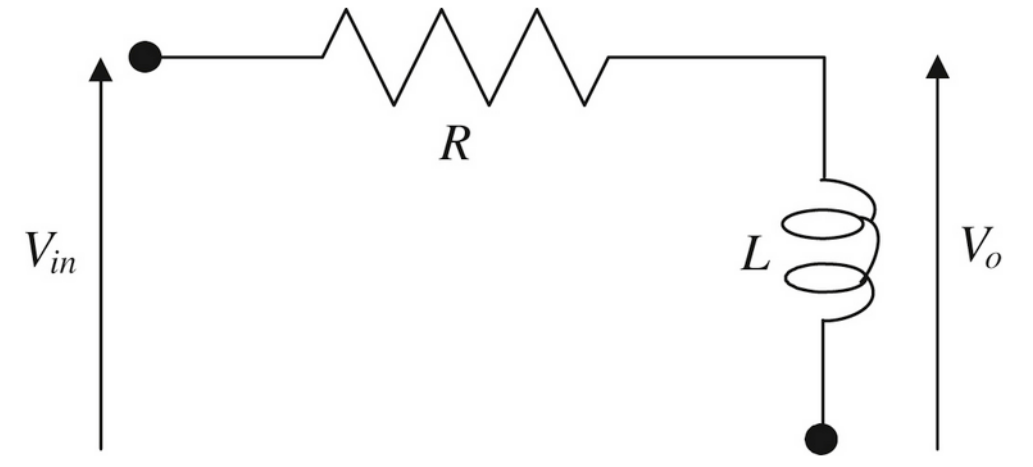
\includegraphics[width=0.8\textwidth]{p1}
\end{figure}
\\
From Example 3.4 of Lecture Notes 3:
  \begin{align*}
    \text{Using the voltage divider rule gives:}\\
    \frac{V_o}{V_{in}} = \frac{Ls}{R+Ls}=\frac{(L/R)s}{1+(L/R)s}=\frac{\tau s}{1+\tau s},\; \tau=\frac{L}{R}\\
    G_{ZAS}(z) = (1-z^{-1})\mathcal{Z}\left\{\frac{1}{s+1/\tau}\right\}\\
    =\frac{z-1}{z}\times\frac{z}{z-e^{-T/\tau}}=\frac{z-1}{z-e^{-T/\tau}}
  \end{align*}
\end{problem}
\pagebreak
\begin{problem}{2}
    Find the steady-state position error for the digitally controlled DC motor with unity-feedback and make sure to \underbar{explain your results}.
    $$G_{ZAS}(z)=\frac{K(z+a)}{(z-1)(z-b)},\;C(z) = K_c\frac{(z-b)}{(z-c)}$$
    $$0<a,b,c<1$$
    From Example 3.10 of textbook (p. 78):
    \begin{enumerate}[label=(\alph*)]
        \item Due to a sampled unit step.
        \begin{align*}
            \text{The loop gain of the system is given by:}\\
            L(z) = C(z)G_{ZAS}(z)=\frac{KK_c(z+a)}{(z-1)(z-c)}\\
            \text{The system is type 1 (only one pole at unity)}.\\
            \text{Therefore, it has 0 steady-state error for unit step.}
        \end{align*}
        \item Due to a sampled unit ramp input.
        \begin{align*}
            \text{The finite steady-state error for a sampled ramp input is given by:}\\
            e(\infty) = \frac{T}{(z-1)L(z)|_{z=1}}=\frac{T}{KK_c}\left(\frac{1-c}{1+a}\right)\\
            \text{This steady-state error can be reduced by increasing the controller gain}\\ 
            \text{and is also affected by the choice of controller pole and zero}
        \end{align*}
    \end{enumerate}
\end{problem}
\pagebreak
\begin{problem}{3}
    Find the state equations given the following simulation diagram:
    \begin{figure}[h]
        \centering
        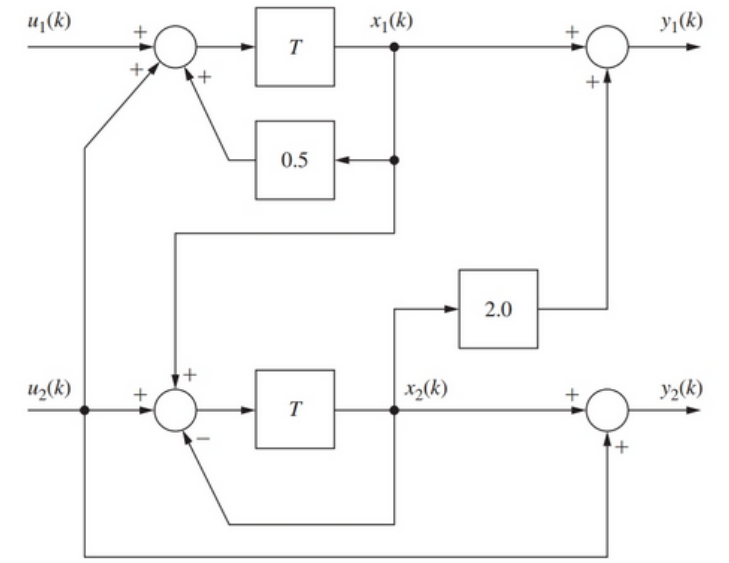
\includegraphics[width=0.8\textwidth]{p3}
    \end{figure}
    \begin{align*}
        x_1(k+1) = T[u_1(k)+u_2(k)+0.5x_1(k)]\\
        x_2(k+1) = T[x_1(k)+u_2(k)-x_2(k)]\\
        y_1(k) = x_1(k)+2.0x_2(k)\\
        y_2(k) = x_2(k)+u_2(k)
    \end{align*}
\end{problem}
\pagebreak
\begin{problem}{4}
    Given
    $$G(z) = \frac{N(z)}{D(z)}$$
    where
    $$D(z) = z^3-z^2-0.2z+0.1$$
    Use the Routh-Hurwitz criterion to find the number of $z$-plane poles of $G(z)$ inside, outside, and on the unit circle. Is the system stable?\\
    From Example 4 of Lecture Note 5A:
    \begin{align*}
        \text{Use the bilinear transformation equation for $D(z)=0$:}\\
        z=\frac{s+1}{s-1}\\
        \text{We get:}\\
        s^3-19s^2-45s-17=0
    \end{align*}
    \begin{table}[h]
        \caption{Routh Table}
        \begin{center}
        \begin{tabular}{|c|c|c|}
        \hline
        \textbf{$s^3$} & 1 & -45 \\
        \hline
        \textbf{$s^2$} & -19 & -17 \\
        \hline
        \textbf{$s^1$} & -45.89 & 0 \\
        \hline
        \textbf{$s^0$} & -17 & 0 \\
        \hline
        \end{tabular}
        \end{center}
      \end{table}
      \\
      One sign change in the first column $\implies$ one root in the R.H.P and two roots in the L.H.P in the $s$-plane.\\
      $\implies$ G(z) has one pole outside the unit circle, no poles on the unit circle, and two poles inside the unit circle\\
      $\implies$ system is unstable because of the pole outside the unit circle.
\end{problem}
\pagebreak
\begin{problem}{5}
    Find the stable range of the gain $K$ for the unity-feedback digital control system with analog plant
    $$G(s) = \frac{K}{s+3}$$
    with DAC and ADC if the sampling period is 0.02 seconds.\\
    From Example 4.7 of the textbook (p. 107):\\
    The transfer function for analog subsystem ADC and DAC is:
    $$G_{ZAS}=(1-z^{-1})\mathcal{Z}\left\{\mathcal{L}^{-1}\left[\frac{G(s)}{s}\right]\right\}$$
    $$=(1-z^{-1})\mathcal{Z}\left\{\mathcal{L}^{-1}\left[\frac{K}{s(s+3)}\right]\right\}$$
    Using the partial fraction expansion
    $$\frac{K}{s(s+3)} = \frac{K}{3}\left[\frac{1}{s}-\frac{1}{s+3}\right]$$
    we obtain the transfer function
    $$G_{ZAS}(z) = \frac{1.9412\times10^{-2}K}{z-0.9418}$$
    For unity feedback, the closed-loop characteristic equation is:
    $$1+G_{ZAS}(z)=0$$
    which can be simplified to
    $$z-0.9418+1.9412\times10^{-2}K=0$$
    The stability conditions are
    $$0.9418-1.9412\times10^{-2}K<1$$
    $$-0.9418+1.9412\times10^{-2}K<1$$
    Thus, the stable range of K is
    $$-3 < K < 100.03$$
\end{problem}
% --------------------------------------------------------------
%     You don't have to mess with anything below this line.
% --------------------------------------------------------------
 
\end{document}